%\normalsize
In the era of the Higgs discovery and extensive searches
for signals of new physics at the LHC it is crucial
to have accurate Standard Model (SM) predictions for
hard scattering processes at the LHC.
The most common approach to calculate the SM cross sections for  
such reactions is to use collinear factorisation in perturbative QCD (pQCD):
%is with perturbative QCD using a (collinear) factorisation approach: 
%{\small
\begin{equation}
\small
\begin{array}{lcl}
\sigma^{pp\rightarrow H + X}(\alpha_s,\mu_r,\mu_f) & = &
\sum\limits_{a,b}\,  \int\limits_{0}\limits^{1} dx_1 \int\limits_{0}\limits^{1} dx_2\, f_a(x_1,\alpha_s,\mu_F) 
 f_b(x_2,\alpha_s,\mu_F)\\ 
& \times & \, \hat{\sigma}^{ab \rightarrow H + X}(x_1,x_2;\alpha_s,\mu_R,\mu_F).
%\sigma^{pp\rightarrow H + X}(\alpha_s,\mu_r,\mu_f) = 
%\sum_{a,b} \int_{0}^{1} dx_1 \int_{0}^{1} dx_2 f_a(x_1) 
% f_b(x_1,\alpha_s,\mu_F) \times \hat{\sigma}^{ab \rightarrow H + X}(x_1,x_2;\alpha_s,\mu_R,\mu_F)
\label{eq:fact}
\end{array}
\end{equation}
%}
Here the cross section $\sigma^{pp\rightarrow H + X}$ for inclusive
Higgs production is expressed
as a convolution of Parton Distribution Functions (PDF) $f_a$ and $f_b$
with the partonic cross section
% that describe
%the 
$\hat{\sigma}^{ab \rightarrow H + X}$.
%
The PDFs describe 
the probability of finding a specific parton $a$ ($b$) in the first (second) proton carrying a fraction $x_1$ ($x_2$) of its momentum.
%
The sum over indices $a$ and $b$ in Eq.~\ref{eq:fact} indicates the various 
kinds of partons,
i.e. gluons and quarks and antiquarks of different flavours, 
that are considered
as the constituents of the proton.
%
Both the PDFs and the partonic cross section depend on the strong coupling
constant $\alpha_s$, and the factorisation and renormalisation scales,
$\mu_F$ and $\mu_R$, respectively.
%
The partonic cross sections are calculable in pQCD, but
the PDFs cannot yet be predicted in QCD, they must rather be 
determined from measuement. They are assumed 
to be universal such that different scattering reactions can be used 
to constrain them; in particular one can use specific reaction data 
for determining the PDFs and then use these PDFs for
predicting other processes.
% via Eq.~\ref{eq:fact}.
%

The Deep Inelastic Scattering (DIS) data from the $ep$ collider HERA provides crucial information for determining the PDFs.
%
For instance, the gluon density relevant
for calculating the dominant gluon-gluon fusion contribution to the Higgs production
at the LHC can be accurately determined from the HERA data alone.
%
%Despite being often plagued by larger perturbative uncertainties,
Specific data from the Tevatron $p\bar{p}$ and the LHC $pp$ collider
can help to further constrain the PDFs.
%
The most sensitive processes at the  colliders are
Drell Yan production, W and Z asymmetries, associated production of W or Z boson 
and heavy quarks, top quark production and jet production.
%

\fitter represents a QCD analysis framework that aims at 
determining precise PDFs by integrating all the PDF sensitive information
from HERA, the Tevatron and the LHC.
%
The processes that are currently included in \fitter framework are listed in Tab.~\ref{tab:proc}.
%
\begin{table}
\small
%\tiny
\scriptsize

\begin{tabular}{|l|l|l|l|}
\hline
Data &Type &  Reaction & Theory      \\
        &     &     & calculation \\
\hline

HERA &DIS NC   &$ep\to ep$      & QCDNUM~\cite{qcdnum}, RT~\cite{Thorne:1997ga,Thorne:2006qt,Martin:epC63,Thorne:6180}, \\
     &         &                & ACOT~\cite{CWZ} \\
HERA &DIS CC   &$ep\to \nu_e p$ & QCDNUM~\cite{qcdnum}, RT~\cite{Thorne:1997ga,Thorne:2006qt,Martin:epC63,Thorne:6180}, \\
     &         &                & ACOT~\cite{CWZ} \\
HERA &DIS jets &$ep\to eX$      & FastNLO (NLOJet++~\cite{Nagy:1998bb,Nagy:2001fj})\\
HERA &DIS heavy                 & $ep\to ep $& ZM (QCDNUM~\cite{qcdnum}), \\
     & quarks  &                & RT~\cite{Thorne:1997ga,Thorne:2006qt,Martin:epC63,Thorne:6180}, ACOT~\cite{CWZ}, \\
     &         &                & FFNS (ABM~\cite{Alekhin:runm,openqcdrad:page}, \\
     &         &                & QCDNUM~\cite{qcdnum}) \\
\hline
Fixed Target   &DIS NC          &$ep\to ep$ & ZM (QCDNUM~\cite{qcdnum}), \\
     &         &                & RT~\cite{Thorne:1997ga,Thorne:2006qt,Martin:epC63,Thorne:6180}, ACOT~\cite{CWZ} \\
\hline
Tevatron, LHC &Drell Yan &$pp(\bar p)$ & APPLGRID (MCFM~\cite{Campbell:1999ah,Campbell:2000je,Campbell:2010ff}) \\
Tevatron, LHC &W charge asym &$pp(\bar p)$ & APPLGRID (MCFM~\cite{Campbell:1999ah,Campbell:2000je,Campbell:2010ff}) \\
Tevatron, LHC &top &$pp(\bar p)$  & APPLGRID (MCFM~\cite{Campbell:1999ah,Campbell:2000je,Campbell:2010ff}),  \\
              &    &              & HATHOR~\cite{Aliev:2010zk} \\
Tevatron, LHC &jets &$pp(\bar p)$ & APPLGRID (NLOJet++~\cite{Nagy:1998bb,Nagy:2001fj}) \\
                &  & & FastNLO (NLOJet++~\cite{Nagy:1998bb,Nagy:2001fj}) \\
LHC& DY + heavy &$pp(\bar p)$ & APPLGRID (MCFM~\cite{Campbell:1999ah,Campbell:2000je,Campbell:2010ff}) \\
   & quarks     &                 & RT~\cite{Thorne:1997ga,Thorne:2006qt,Martin:epC63,Thorne:6180}, ACOT~\cite{CWZ}, \\
\hline
\end{tabular}
\caption{The list of processes available in the \fitter package. 
The APLLGRID~\cite{Carli:2010rw} and FastNLO~\cite{Kluge:2006xs,Wobisch:2011ij,Britzger:2012bs} 
techniques for the fast interface to theory calculations are described in section~\ref{sec:techniques}.} 
\label{tab:proc}
\end{table}
%
\normalsize
The basic functionality of HERAFitter is shown in Fig.~\ref{fig:flow} and consists of four parts: %{\bf needs to update figure!}
\begin{figure}[!ht]
  \begin{tikzpicture}[node distance=1cm, auto,>=latex', thick]
      \path[->] node[draw, text width=2cm, align=center] at (0,0) (init) {\bf Initialization};
      \path[->] node[draw, below left=0.3cm and -0.7cm of init, text width=3.5cm] (data) 
                    {\begin{center} \vspace{-0.3cm}{\bf Input Data} 
		      \\ {\color{blue}\small Data Type} 
		     \end{center} 
		     {\scriptsize 
		     \begin{itemize}
                      \vspace{-0.3cm}
		      \item Collider ep
		      \item Collider pp
		      \item Fixed target data
		     \end{itemize}}
		     } (init) edge (data);
      \path[->] node[draw, below right=0.3cm and -0.7cm of init, text width=3.5cm] (theory) 
                    {\begin{center} \vspace{-0.3cm}{\bf Theory Predictions} 
		      \\ {\color{red}\small Factorization Theorem} 
		     \end{center} 
		     {\scriptsize 
		     \begin{itemize}
                      \vspace{-0.3cm}
		      \item PDF Parametrisation
		      \item QCD Evolution (QCDNUM)
		      \item Cross Section Calculation
		     \end{itemize}}
		     } (init) edge (theory);
      \path[->] node[draw, below right=0.4cm and -1.4cm of data, text width=3.5cm] (minuit) 
                    {\begin{center} \vspace{-0.3cm}{\bf Minimisation (MINUIT)} 
                      \vspace{-0.2cm}
		     \end{center} 
		     {\color{blue}\scriptsize Treatment of the uncertainties:} 
		     {\scriptsize 
                      \vspace{-0.1cm}
		     \begin{itemize}
		      \item PDF Parametrisation
		      \item QCD Evolution (QCDNUM)
		      \item Cross Section Calculation
		     \end{itemize}}
		     } (data) edge (minuit)
		     (theory) edge (minuit)
		     (data) ++ (1.6,0) edge [<->,double equal sign distance] ++(1.36,0) (theory);
      \path[->] node[draw, below =0.4cm  of minuit, text width=3.5cm] (res) 
                    {\begin{center} \vspace{-0.3cm}{\bf Results} 
		     \end{center} 
		     {\scriptsize 
		     \begin{itemize}
                      \vspace{-0.3cm}
		      \item PDF LHgrids
		      \item alphas, mc, \dots
		      \item Data vs Predictions
		      \item \(\chi^2\), pulls, shifts
		     \end{itemize}}
		     } (minuit) edge (res);
  \end{tikzpicture}
  \caption{Schematic structure of the \fitter program.} 
  \label{fig:flow}
\end{figure}

%\begin{figure}[!ht]
%   \centering
%   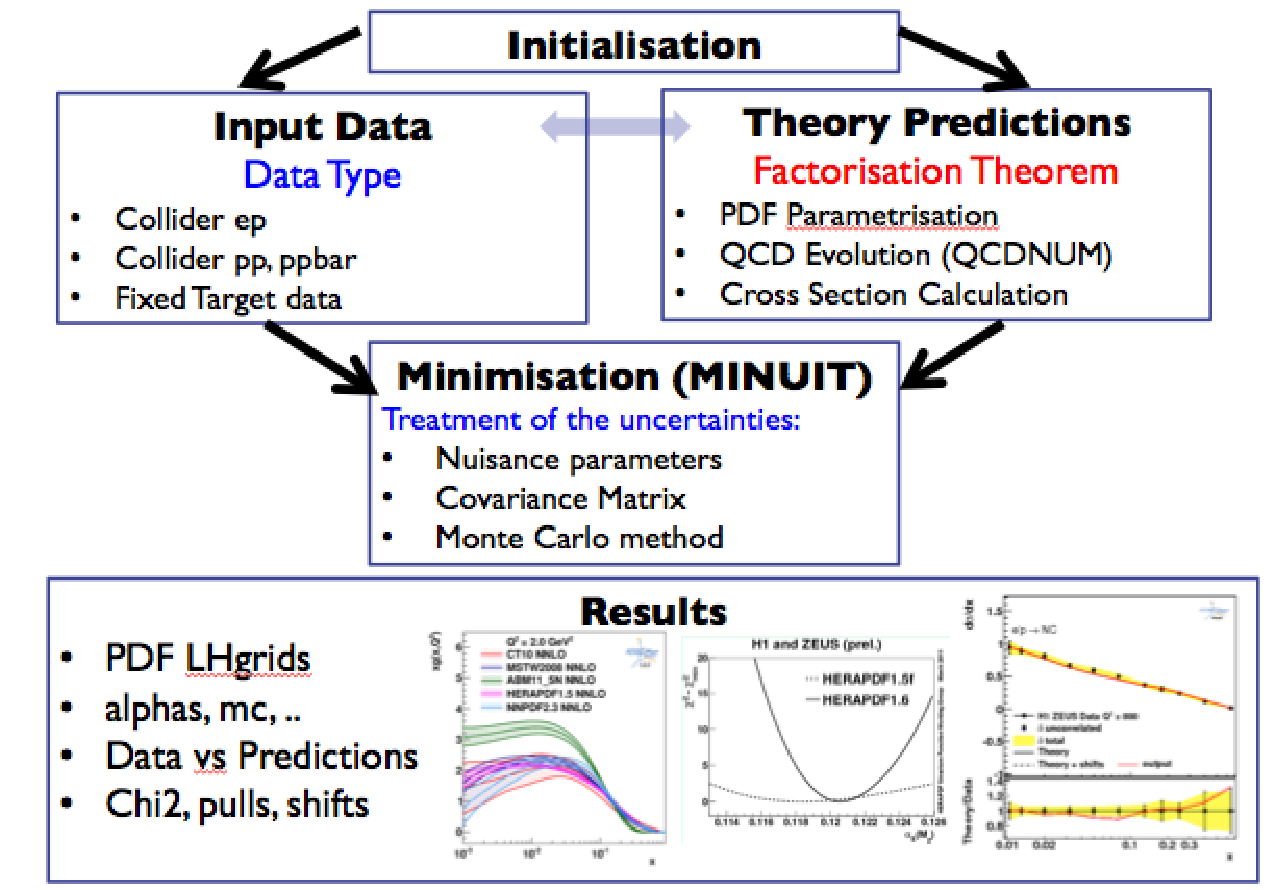
\includegraphics[width=8cm]{flow.pdf}
%   \caption{Schematic structure of the \fitter program.} 
% \label{fig:flow}
%\end{figure}
\begin{description}
\item 
\bf {Input data:} \rm  All relevant cross section data from the various reactions
are stored internally in \fitter with the full information on their uncorrelated and correlated
uncertainties.
\item
\bf{Theory predictions:} \rm Predictions are obtained relying on the factorisation approach (Eq.~\ref{eq:fact}). PDFs are parametrised at a starting scale $Q_0$  by a chosen functional form with a set of free parameters $\vec{p}$. They are then evolved from $Q_0$ to the scale of the measurement using the 
Dokshitzer-Gribov-Lipatov-Altarelli-Parisi 
(DGLAP)~\cite{Gribov:1972ri, Gribov:1972rt, Lipatov:1974qm,
Dokshitzer:1977sg, Altarelli:1977zs} evolution equations 
as implemented in QCDNUM~\cite{qcdnum}, 
and then convoluted (Eq.~\ref{eq:fact}) with the hard parton cross sections calculated by
a specific theory program (as listed in Tab.~\ref{tab:proc}).
\item
\bf{Minimization:} \rm  PDFs are extracted from a least square fit by constructing a 
$\chi^2$ from the input data and the theory prediction.
The $\chi^2$ is  minimized iteratively 
with respect to the PDF parameters using the MINUIT\cite{minuit} program.
%
%Fitted values of $\vec{p}$ and estimated uncertainties are obtained.
%The fitted parameters $\vec(p)$ and obtained from the uncertainties of the parameters are determined (from chi2+1???)
%
\item
\bf{Results:} \rm  The fitted parameters $\vec{p}$ and their estimated uncertainties are produced.
The resulting PDFs are provided in a format ready to be used by the LHAPDF 
library~\cite{lhapdf,lhapdfweb}. Tools are supplied which allow the PDFs to be
graphically 
displayed at arbitrary scales with their one sigma uncertainty bands.
To demonstrate the fit consistency, plots 
which compare the input data to the fitted theory predictions can be made using
tools supplied with the package. 
This is illustrated in the Fig.~\ref{fig:data} showing  
HERA~I data (the default data set in \fitter) compared to predictions based on 
HERAPDF1.0\cite{h1zeus:2009wt}. This figure also illustrates this comparison 
taking into account the systematic uncertainty shift parameters which are 
applied to the predictions in the nuisance parameter method of accounting for 
correlated systematic uncertainties (see section~\ref{sec:chi2representation}) and the pulls 
as an additional consistency check between data and the theory prediction 
(defined as the difference between data and prediction divided by the uncorrelated uncertaintly of the data).
\begin{figure}[!ht]
   \centering
   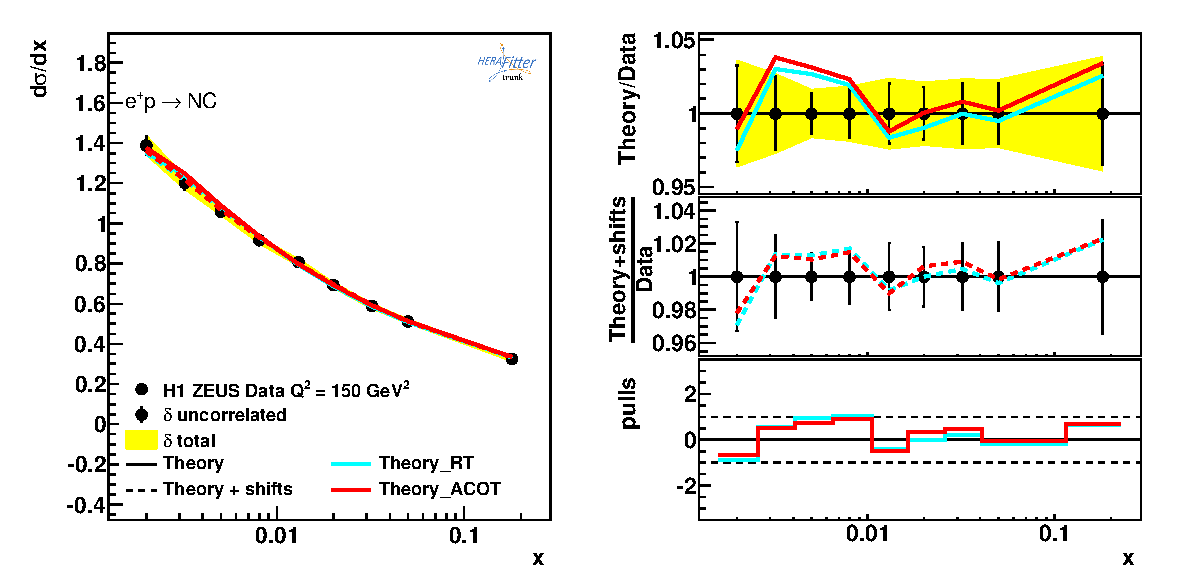
\includegraphics[width=8cm]{datatheory.pdf}
   \caption{An illustration of the \fitter drawing tools comparing the measurements (in this case HERA I) to the predictions of the fit. In addition, ratio plots are also provided together with the pull distribution (right panel).} 
 \label{fig:data}
\end{figure}

\end{description}
%
%This paper provides a comprehensive description of  \\
%the \fitter\ package.
%which is designed for analysis of the High Energy Physics data.
%The package has been developed by members of the H1 and ZEUS collaborations
%with an exclusive support of different theoretical groups.
%The main purpose of the \fitter\ package is analysis of the 
%data from the $e^{\pm}p$, $p\bar{p}$, and $pp$ collider experiments
%information obtained from the deep inelastic scattering experiments
%and the determination of the parton density functions (PDFs).
%The broad range of data taken from the $e^{\pm}p$, $p\bar{p}$, and $pp$ collider experiments can be
%studied by the package. 

%Based on the concept of factorisable nature of the cross sections into universal parton distribution functions (PDFs) and process dependent partonic scattering cross sections, 

The \fitter\ program facilitates the determination of the PDFs from many 
cross section measurements at $ep$, $p\bar{p}$ or $pp$ colliders.  
 It includes various options for theoretical calculations and various choices 
of how to 
account for the experimental uncertainties. Therefore, this project represents 
an ideal environment for benchmarking studies and a unique platform for the QCD interpretation of analyses within the LHC experiments,
as already demonstrated by several publicly available results using the \fitter\ 
framework~\cite{atlas:strange,atlas:jets,atlas:hm,cms:strange,cms:jets,h1:2012kk,h1zeus:charm}.  

The outline of this paper is as follows.
%
Section~\ref{sec:theory} discusses the various processes 
and corresponding theoretical calculations performed in the DGLAP~\cite{Gribov:1972ri,Gribov:1972rt,Lipatov:1974qm,
Dokshitzer:1977sg,Altarelli:1977zs} formalism that are available in \fitter.
Alternative approaches to the DGLAP formalism are presented in section~\ref{sec:alternative}.
%
In section~\ref{sec:techniques} various different choices made in the 
theory calculations are described.
Section~\ref{sec:method} elucidates the 
methodology of determining PDFs through fits based on various
% {\bf (what do you mean here
%by approaches?)} 
 $\chi^2$ definitions used in the
minimisation procedure. 
%
Specific applications of the package are given in
section ~\ref{sec:examples}. 
%
%{\bf add something more here?.}
